\subsection{Background}
In laminar flow problems, the lift and drag coefficients play a crucial role in characterizing the aerodynamic behavior of an object in relative motion with a fluid. These coefficients are dimensionless parameters and are directly proportional to the lift and drag forces experienced by an object, and inversely proportional to the square of the reference relative velocity.

\subsubsection{Lift Coefficient}
The lift coefficient represents the efficiency of an airfoil or any aerodynamic shape in generating lift perpendicular to the direction of flow. In laminar flow, understanding the lift coefficient is essential for predicting the upward force that counters the weight of an object (e.g., an aircraft wing).
\subsubsection{Drag Coefficient}
The drag coefficient characterizes the resistance an object experiences parallel to the flow direction. In laminar flow, it is critical for estimating the drag force opposing the object's motion through the fluid.
    
\subsection{Calculation}
\subsubsection{Equations in the benchmark}
According to the definitions given in the suggested paper \cite{Cylinder}, the lift and drag forces are:
\begin{equation}
F_L = - \int_S (\rho \nu \frac{\partial v_t}{\partial n}n_x + P n_y) \, dS
\end{equation}
\begin{equation}
F_D = \int_S (\rho \nu \frac{\partial v_t}{\partial n}n_y - P n_x) \, dS
\end{equation}
With the following notation: $\mathcal{S}$ (a circular curve in two dimensions, and a capless cylinder's surface in three dimensions), normal vector $\mathbf{n}$ on $\mathcal{S}$ with x-component $n_x$ and y-component $n_y$, tangential velocity $v_t$ on $\mathcal{S}$, pressure $P$ and tangent vector $\mathbf{t} = (n_y, -n_x)$ or $\mathbf{t} = (n_y, -n_x, 0)$, depending on the problem's dimensionality.

After calculating the lift and drag forces, the corresponding lift and drag coefficients are, in the two dimensional case:
\begin{equation}\label{eq:lift_coeff}
    C_L = \frac{2F_a}{\rho \bar{U}^2 D}
\end{equation}
\begin{equation}\label{eq:drag_coeff}
    C_D = \frac{2F_w}{\rho \bar{U}^2 D}
\end{equation}
While in the three dimensional case the equations have an additional $H$ factor in the denominator.

\subsubsection{Issues with the equations}
These definitions suffer from multiple issues: for example, the terms $F_w$ and $F_a$ are never defined in \cite{Cylinder} and the formulae do not match with the ones given in the project description, not even in terms of physical units of measurement. As such, we compared multiple sources in the scientific literature and decided to use the formulae supported by the largest number of reliable sources. 

\paragraph{Lift and drag forces}
Regarding the computation of the lift and drag coefficients utilizing the computed forces, both \cite{Dede} and \cite{lift_drag} provide the same formula as Equation \ref{eq:drag_coeff}, where $F_w$ is the drag force.  For this reason, we decided to use Equations \ref{eq:lift_coeff} and \ref{eq:drag_coeff} and their 3D generalization, using $F_L$ and $F_D$ in place of $F_a$ and $F_w$.

\paragraph{Lift and drag coefficients}
Regarding the calculation of the drag and lift forces, we decided to use the formula for the drag force presented by \cite{Dede}. Said formula is similar to the one used in \cite{lift_drag}, which we used to generalize it to the lift force computation. The formulae we used for both the two and three dimensional cases are therefore:
\begin{equation}\label{eq:lift_force}
    F_L = \int_S \rho ((\nu (\nabla u + \nabla u^T) - p I)\mathbf{n}) \cdot \hat{j} dS
\end{equation}
\begin{equation}\label{eq:drag_force}
    F_D = \int_S \rho ((\nu (\nabla u + \nabla u^T) - p I)\mathbf{n}) \cdot \hat{i} dS
\end{equation}
Where $I$ is the identity tensor, $\hat{i}$ and $\hat{j}$ are the unit vectors in the $x$ and $y$ direction respectively and $\mathbf{n}$ has the same meaning as in the previous equations. The notation in \cite{Dede} and \cite{lift_drag} was not adopted, as to match the notation used in the rest of the report.

\subsubsection{More accurate equations}
The described formulae suffer from one more issue: since we are integrating terms depending on the pressure and on the gradient of the velocity over a boundary with one less physical dimension that $\Omega$, the operation is not well-defined in the weak sense.

\paragraph{New equations}
A method to compute the drag coefficient in two dimensions in a well-defined manner that gives enhanced precision is provided in \cite{Dede}, which we extended to the computation of the lift coefficient and to the three dimensional case. In particular, this method consists in finding two functions $\mathbf{\phi}_\infty^L$ and $\mathbf{\phi}_\infty^D$ in $(H^1(\Omega))^d$ that satisfy the following constraints:
\begin{equation}\label{eq:phi_inf_lift}
    \mathbf{\phi}_\infty^L|_{\mathcal{S}} = -\hat{j} \land \mathbf{\phi}_\infty^L|_{\partial\Omega \setminus \mathcal{S}} = \mathbf{0}
\end{equation}
\begin{equation}\label{eq:phi_inf_drag}
    \mathbf{\phi}_\infty^D|_{\mathcal{S}} = -\hat{i} \land \mathbf{\phi}_\infty^D|_{\partial\Omega \setminus \mathcal{S}} = \mathbf{0}
\end{equation}
And then letting 
\begin{equation}\label{eq:force_weak}
    F = \int_{\Omega} \nu \nabla \mathbf{u} : \nabla \mathbf{\mathbf{\phi}_\infty} \, d\Omega + \int_{\Omega} ((\mathbf{u} \cdot \nabla) \mathbf{u}) \cdot \mathbf{\phi}_\infty \, d\Omega - \int_{\Omega} p \nabla \cdot \mathbf{\phi}_\infty \, d\Omega
\end{equation}
Where $F$ and $\mathbf{\phi}_\infty$ are $F_L$ or $F_D$ and $\mathbf{\phi}_\infty^L$ or $\mathbf{\phi}_\infty^D$ for the lift and the drag forces respectively. 

\paragraph{Discretization}
We then discretized the equation in space, using the same finite element space as for the discrete problem, and looked for two functions $\mathbf{\phi}_{\infty h}^L$ and $\mathbf{\phi}_{\infty h}^D$ which fit Equations \ref{eq:phi_inf_lift} or \label{phi_inf_drag} for all test functions $\mathbf{v}_h$ in $V_h$. Since there are infinitely many functions that meet the conditions, we set the additional constraint:
\begin{equation}
    \int_\Omega \mathbf{\phi}_\infty \mathbf{v}_h \, d\Omega = 0 \; \forall \mathbf{v}_h \in V_h
\end{equation}
Which results in linear systems that can be solved using the already assembled and relatively well-conditioned mass matrix for the velocity and using the lifting technique.

\subsection{Results}\label{sec:lift_drag_plots}
Figure \ref{fig:lift-drag} shows the plot of the lift and drag coefficients over time for the two and three dimensional flow past a cylinder benchmark and multiple values of Reynolds number. 2D results use $\Delta t = 5*10^{-4}s$ and \texttt{-clmax 0.25}, while 3D results use $\Delta t = 10^{-3}s$ and \texttt{-clmax 0.5}. The result for $t = \Delta t$ was removed from the images, as it is out of scale due to the sudden change in the inlet velocity. The black line reports the results obtained with Formulae \ref{eq:lift_force} and \ref{eq:drag_force}, while the red line reports the results obtained with Formula \ref{eq:force_weak}. 3D simulations were run before the implementation of the new formula for calculation of the forces.

\begin{figure}[]
    \centering
    \subfigure[2D problem, Re = 48]{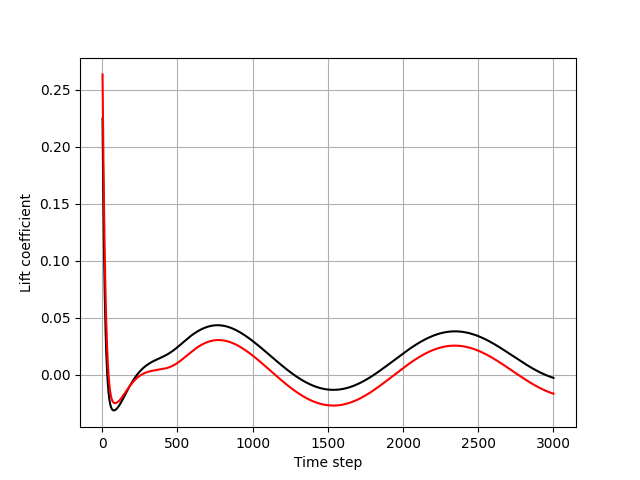
\includegraphics[width=38mm]{image/2d-lift-48}}
    \subfigure[2D problem, Re = 48]{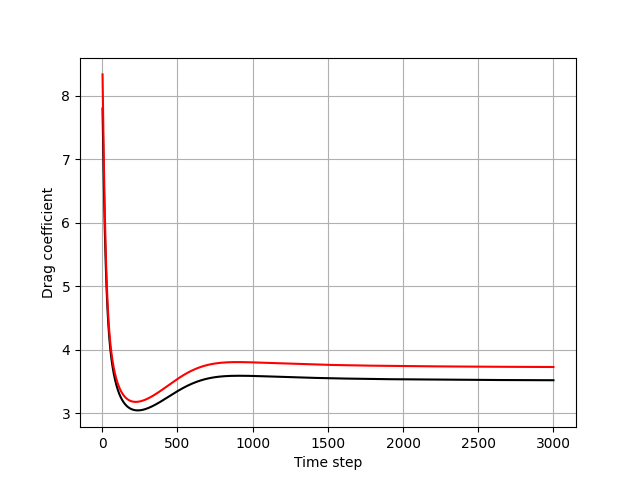
\includegraphics[width=38mm]{image/2d-drag-48}}
    \subfigure[2D problem, Re = 200]{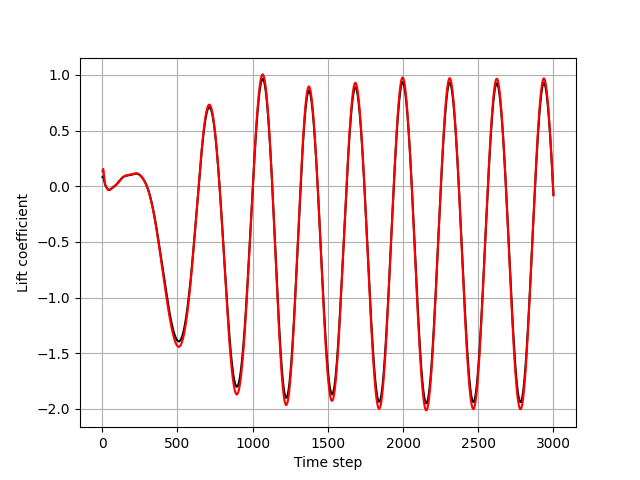
\includegraphics[width=38mm]{image/2d-lift-200}}
    
    \subfigure[2D problem, Re = 200]{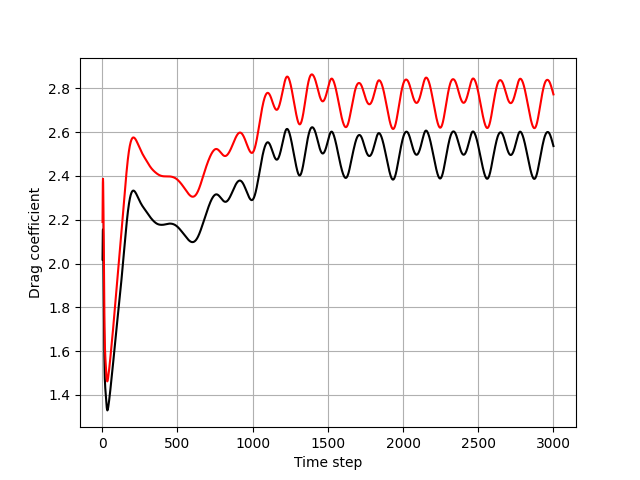
\includegraphics[width=38mm]{image/2d-drag-200}}
    \subfigure[3D problem, Re = 133]{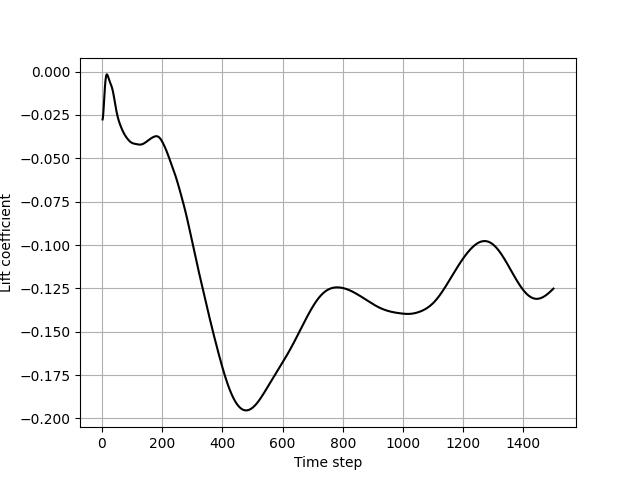
\includegraphics[width=38mm]{image/3d-lift-3.0}}
    \subfigure[3D problem, Re = 133]{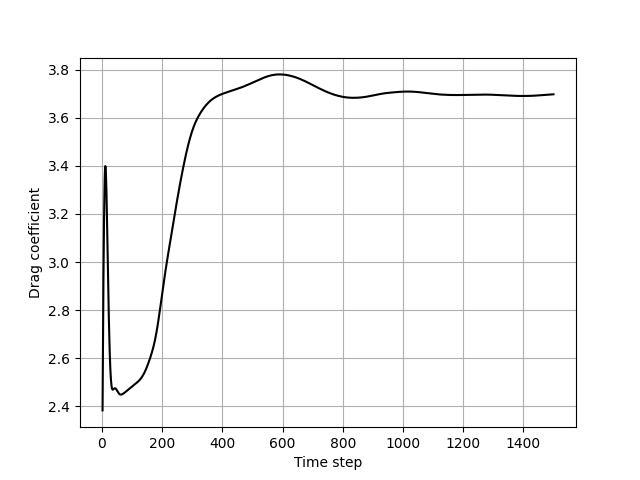
\includegraphics[width=38mm]{image/3d-drag-3.0}}
    
    \caption{Plot of lift and drag coefficients over time for the test case with constant inlet velocity. On the $x$ axis, the time step $n$ is reported, where $t = n\Delta t$.}
    \label{fig:lift-drag}
\end{figure}

\subsection{Results discussion}
While we were unable to find results for our exact test, multiple sources in the scientific literature show a qualitative behaviour of the lift and drag coefficients similar to ours for similar problems \cite{lift_drag}\cite{lift_drag_2}\cite{lift_drag_3}. Namely, the lift coefficient oscillates over time, with a frequency that increases with the Reynolds number, while the drag coefficient starts at a high value, decreases to a minimum and then increases again, with small oscillations for Re = 200.

We tested other configurations of Reynolds numbers, both in 2D and 3D, but did not include the results for the sake of brevity. Regarding the test case with a time dependent inlet velocity, in this test case the Reynolds number is a sine wave with semiperiod $8s$. As expected, when the time tends to $0$ or to $8s$, the absolute value of the drag coefficient tends to infinity, as it is inversely proportional to the Reynolds number for small values of Re.